%_____________________________________________________________________________________________
% Chapter 3: Problem Definition and Requirements
%_____________________________________________________________________________________________

\chapter{Problem Definition and Requirements}
\label{ch:problem}

\section{Formal Problem Setting}
A frozen binary classifier $f$ is trained on a labeled reference set $R$ and then scores a stream of batches $B_0, B_1, B_2, \dots$ of 300 rows each. The monitor sees the rows of every batch and the predictions of $f$ immediately. The true labels of batch $b$ become usable at batch $b+\max(L,1)$, where $L$ is the label delay (primary setting $L=5$). The first 8 batches after deployment form a \emph{burn-in} period during which no alerts are raised; the monitor uses them to learn what normal looks like for this stream.

\subsection{Degradation event}
The baseline accuracy is the mean accuracy of $f$ on batches 0--4. A \emph{degradation event} begins at the first of two consecutive batches whose accuracy is at least 5 percentage points below the baseline. Requiring two consecutive batches avoids calling a single noisy batch an event.

\subsection{Episodes and outcomes}
An \emph{episode} is one monitored stream of 45 batches. In controlled episodes an intervention starts at a known batch $s$. Each shift episode is then labelled from the true accuracy:
\begin{itemize}
\item \textbf{Harmful}: an event starts at or after $s$;
\item \textbf{Harmless}: no event occurs;
\item \textbf{Spurious}: an event starts before $s$ (or occurs in a clean episode); spurious episodes are excluded from the main hypotheses and their number is reported.
\end{itemize}

\subsection{Warning tiers}
For an intervention at batch $s$ and an event at batch $e$ we distinguish three tiers (\figref{fig:tiers}):
\begin{itemize}
\item \textbf{T1, predictive warning}: an alert in $[s, e)$, before the accuracy actually drops. The \emph{lead time} is $e$ minus the first such alert.
\item \textbf{T2, pre-confirmation warning}: an alert in $[s, e+1+\max(L,1))$, before delayed labels could confirm the event. In practice T2 matters most, because it measures what the monitor adds over waiting for labels.
\item \textbf{T3, confirmed}: the first alert at or after confirmation; by then the labels already show the drop.
\end{itemize}

\begin{figure}[H]
\centering
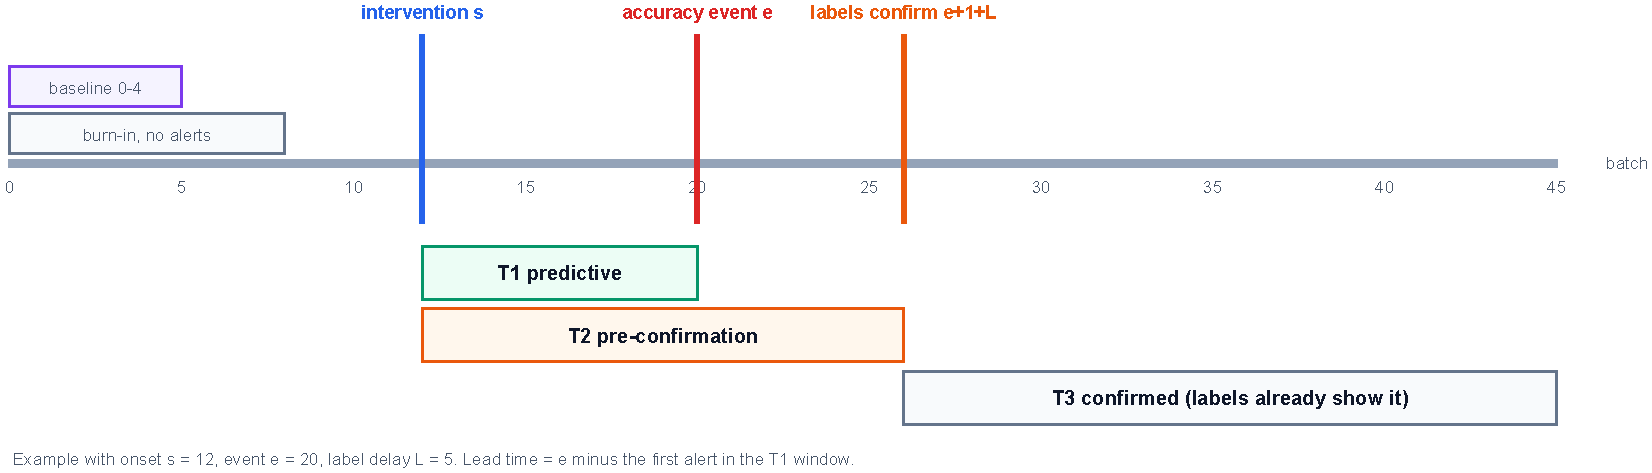
\includegraphics[width=\textwidth]{fig_warning_tiers.pdf}
\caption{Warning tiers on the batch axis, for onset $s=12$, event $e=20$ and label delay $L=5$. T1 ends when accuracy drops; T2 ends when delayed labels could confirm the drop.}
\label{fig:tiers}
\end{figure}

\subsection{False alerts}
\emph{Clean batches} are all batches of unshifted (clean) episodes and the pre-intervention batches of every other episode. The \emph{false-alert rate} is the number of alerts on clean batches per 100 clean batches, with a budget of \textbf{5}. For harmless shifts, which never cause an event, we report the \emph{harmless-alarm share}: the share of harmless episodes with any alert after onset.

\subsection{Separation of harm}
To measure whether a score separates harmful from harmless shifts, we take its mean over the first 3 batches after onset in each shift episode and compute the area under the ROC curve (AUROC) between harmful and harmless episodes. An AUROC of 0.5 means no separation; 1.0 means perfect separation.

\section{Functional Requirements}
\begin{enumerate}[label=FR\arabic*.]
\item \textbf{Stream construction.} Build monitored episodes from any binary tabular OpenML dataset: reference set, pool, 45 batches, controlled shifts with a known onset, and true labels for every row.
\item \textbf{Signal extraction.} For every batch, compute label-free signals: per-feature drift statistics, the fused DEWS drift score, relevance-weighted shift, positive-rate shift, confidence, entropy, and disagreement with auxiliary models.
\item \textbf{Delayed labels.} Release the labels of batch $b$ only at batch $b+\max(L,1)$; never let a score at batch $t$ use a label that has not matured.
\item \textbf{Drift watch.} Normalise every signal against the stream's burn-in and raise a WATCH alert when the largest normalised signal exceeds the frozen threshold.
\item \textbf{Harm tier.} Estimate the model's current accuracy from the labeled reference set by importance weighting and raise a HARM alert when the estimated drop exceeds the frozen threshold.
\item \textbf{Confirmation.} When delayed labels arrive, confirm or clear the warning with the event rule.
\item \textbf{Evaluation.} Compute T1, T2, T3, lead times, false-alert rates, harmless-alarm shares and AUROC with bootstrap confidence intervals.
\item \textbf{Pre-registration.} Freeze thresholds and rules in versioned configuration files with SHA-256 fingerprints, and refuse to run a confirmation if a fingerprint does not match.
\item \textbf{Verdicts.} Apply the frozen pass rules mechanically and write a verdict file and report.
\item \textbf{Dashboard.} Replay a saved episode batch by batch with a chosen label delay, show both tiers and the delayed labels, explain which signals moved, and show all verdicts and ablations.
\end{enumerate}

\section{Non-Functional Requirements}
\begin{enumerate}[label=NFR\arabic*.]
\item \textbf{Causality.} No score may use future labels or event outcomes; this is enforced in code and covered by unit tests.
\item \textbf{Reproducibility.} Every episode is generated from a recorded seed; all models use fixed random states; bootstrap intervals use fixed generator seeds; a single command rebuilds and verifies the verdicts.
\item \textbf{Honesty of evaluation.} Thresholds are chosen on development data only; confirmation data are downloaded only after the design is frozen; each confirmation is run once.
\item \textbf{Performance.} Monitoring a batch must take well under a second on a laptop; the earlier replay pipeline measured about 0.08 seconds per batch.
\item \textbf{Maintainability.} Code is linted (Ruff), unit-tested (pytest) and checked by continuous integration on Python 3.10, 3.11 and 3.12.
\item \textbf{Usability.} The dashboard must be understandable to a non-specialist examiner in a short demonstration.
\end{enumerate}

\section{Hardware and Software Requirements}
\begin{table}[H]
\caption{Hardware and software used.}
\label{tab:env}
\centering
\small
\begin{tabularx}{\textwidth}{@{}p{3.5cm}X@{}}
\toprule
Item & Specification \\
\midrule
Hardware & Laptop, Intel Core i7-12650H (10 cores, 16 threads), 16 GB RAM; no GPU needed \\
Operating system & Windows 11 (development); Ubuntu (continuous integration) \\
Language & Python 3.10--3.12 (development on 3.12) \\
Core libraries & NumPy 2.5.4, SciPy, pandas 2.3, scikit-learn 1.7.2, statsmodels, matplotlib \\
Dashboard & Streamlit 1.57+, Altair \\
Testing and CI & pytest 8, Ruff 0.17.4, GitHub Actions \\
Data source & OpenML~\cite{vanschoren2014openml}, fetched with scikit-learn \\
Documents & \LaTeX\ (IEEEtran for the paper, this template for the report), draw.io for diagrams \\
Legacy (optional) & FastAPI, uvicorn, MLflow, PostgreSQL drivers, in a separate environment \\
\bottomrule
\end{tabularx}
\end{table}

\section{Users and Use Cases}
Two kinds of users interact with the system (\figref{fig:usecases}). An \emph{ML engineer} uses the monitor and the dashboard to see whether a deployed model is drifting and whether the drift is likely to hurt it. A \emph{researcher or examiner} reads the verdicts, reproduces them, and runs new pre-registered experiments. OpenML acts as an external system that supplies datasets.

\begin{figure}[H]
\centering
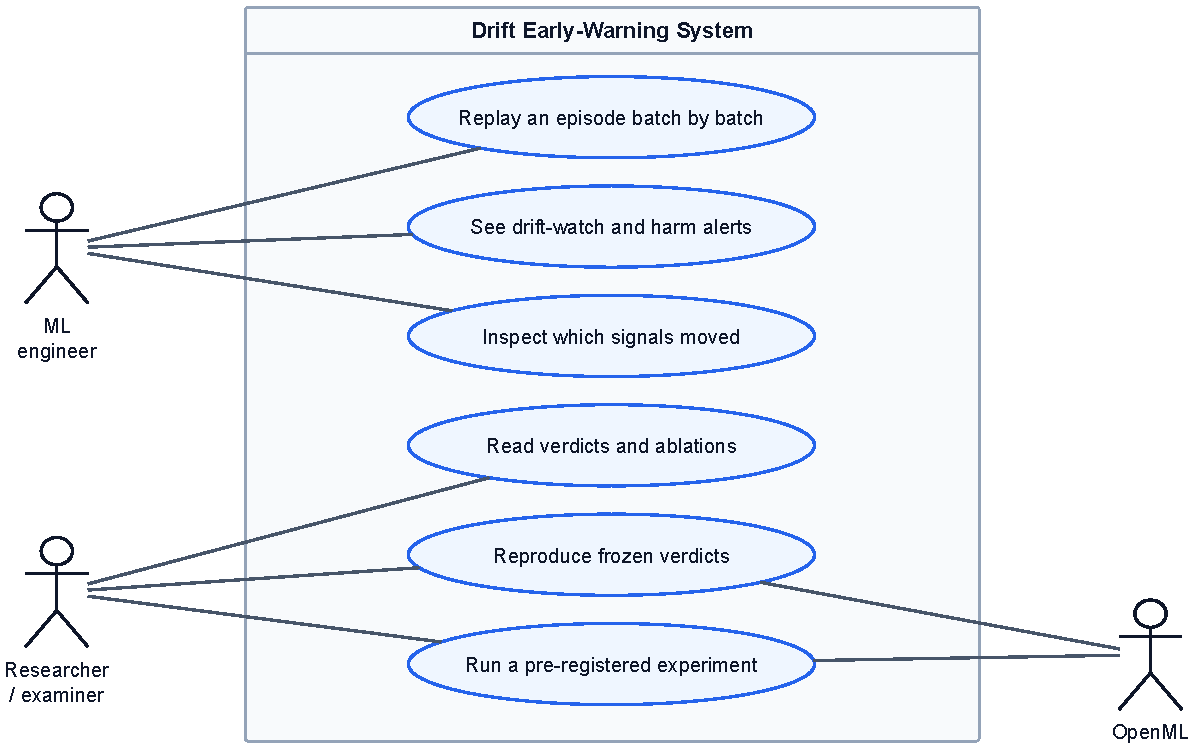
\includegraphics[width=0.8\textwidth]{fig_usecases.pdf}
\caption{Use-case diagram of the Drift Early-Warning System.}
\label{fig:usecases}
\end{figure}
